\documentclass[11pt]{report}

\usepackage{amsmath}
\usepackage{amssymb}
\usepackage{amsfonts}
\usepackage{dsfont}
\usepackage{epsfig}
\usepackage{times}
\usepackage{multicol}
%\usepackage{mcode}

\usepackage{geometry}
\geometry{letterpaper, margin=0.25in}

\usepackage{bm}

\usepackage{footnote}
\makesavenoteenv{tabular}

\usepackage{enumerate}
%\usepackage{enumitem}
\usepackage{pdfpages}
%\usepackage{hyperref}
\usepackage{calc}
\usepackage{verbatim}

\DeclareMathOperator{\Prob}{\mathbb{P}}
\DeclareMathOperator{\Exp}{\mathbb{E}}
\DeclareMathOperator{\Var}{\text{Var}}
\DeclareMathOperator{\SSS}{\mathcal{S}}

\newcommand{\bs}{\boldsymbol}

\newcommand{\be}{\begin{enumerate}}
\newcommand{\ee}{\end{enumerate}}

\newcommand{\teq}{\triangleq}
\newcommand{\tr}{{\text{\tiny T}}}

\parindent = 0cm
\parskip=5pt

\DeclareMathOperator*{\argmax}{\arg\max}
\DeclareMathOperator*{\argmin}{\arg\min}

\newcommand{\ans}[1]{\boxed{\text{#1}}}
\newcommand{\vecs}[1]{\langle #1\rangle}
\renewcommand{\hat}[1]{\widehat{#1}}
\newcommand{\F}[1]{\mathcal{F}(#1)}
\renewcommand{\P}{\mathbb{P}}
\newcommand{\R}{\mathbb{R}}
\newcommand{\E}{\mathbb{E}}
\newcommand{\Z}{\mathbb{Z}}
\newcommand{\ind}{\mathbbm{1}}
\newcommand{\qed}{\quad \blacksquare}
\newcommand{\brak}[1]{\left\langle #1 \right\rangle}
\newcommand{\bra}[1]{\left\langle #1 \right\vert}
\newcommand{\ket}[1]{\left\vert #1 \right\rangle}
\newcommand{\abs}[1]{\left\vert #1 \right\vert}
\newcommand{\mfX}{\mathfrak{X}}

\newcommand{\sub}{\subset}

\renewcommand{\div}{\vspace*{10pt}\hrule\vspace*{10pt}}

\newcommand{\norm}[1]{\left\vert\left\vert #1 \right\vert\right\vert}


\usepackage{tcolorbox}
\tcbuselibrary{breakable, skins}
\tcbset{enhanced}
\newenvironment*{tbox}[2][gray]{
	\begin{tcolorbox}[
		parbox=false,
		colback=#1!5!white,
		colframe=#1!75!black,
		breakable,
		title={#2}
	]}
	{\end{tcolorbox}}


\begin{document}
\begin{center}
	{\bf\large APMA 1740/2610 2025: Homework 5}
\end{center}
%\noindent{\bf\Large BE SURE TO CHANGE TO THE APPROPRIATE HW NUMBER}
\medskip


\begin{enumerate}[1.]

	\item {\bf Softmax: a tale of two loss functions.}
	      \label{item:two_losses}
	      There are two natural ways to measure the performance of a softmax classifier relative to the training data: the likelihood (corresponding to the cross-entropy loss) and the error rate. This problem explores the connections between the cross-entropy
	      and error-rate loss functions in the context of the softmax model.

	      Consider a classification problem with feature vectors $x\in \mathds{R}^d$ and categories $y\in\{1,2,\ldots,s\}$.
	      Given training data
	      $(x_k,y_k)$, $k=1:n$, suppose that we adopt the softmax model, i.e.
	      \[
		      r_c(x;\beta_1,\ldots,\beta_s)  = \mathds{P}\left(Y=c\big|x;\beta_1,\ldots,\beta_s\right) = \frac{ e^{\beta_c\cdot x} }{ \sum_{\tilde{c} = 1}^s e^{\beta_{\tilde c}\cdot x} }\quad \forall\ c=1:s
	      \]
	      To avoid over-parametrization, we define $\beta_1 \triangleq 0$.

	      Consider the Bayes (minimum-error) classifier:
	      \[
		      h(x;\beta_2,\ldots,\beta_s)  = \text{argmax}_c \mathds{P}\left(Y=c\big|x;\beta_2,\ldots,\beta_s\right)
	      \]

	      Assume that the data is consistent, i.e. $x_k = x_l \Rightarrow y_k=y_l$, and that every category is represented, i.e. for every $c$ there exists a $k$ such that $y_k=c$.

	      \begin{enumerate}[(a)]
		      \item Show that the error rate on the training data is zero (i.e. $h(x_k) = y_k$ for all $k=1:n$) if and only if, for every $k=1:n$,
		            \[
			            (\beta_{y_k} - \beta_c)\cdot x_k > 0\quad \text{for all $c\neq y_k$}
		            \]

		            \color{blue}
		            ($\implies$). By assumption,
		            \begin{align*}
			            h(x_k; \beta_2, \dots, \beta_s) = \argmax_c \P(Y = c \; | \;  x_k; \beta_2, \dots, \beta_s) \\
			            = \argmax_c r_c(x_k; \beta_1, \dots, \beta_s)                                               \\
			            = \argmax_c \frac{e^{\beta_c \cdot x_k}}{\sum_{\tilde{c} = 1}^s e^{\beta_{\tilde c} \cdot x_k}} = y_k
		            \end{align*}

		            But this means that for any $c \neq y_k$,
		            \[\frac{e^{\beta_c \cdot x_k}}{\sum_{\tilde{c} = 1}^s e^{\beta_{\tilde c} \cdot x_k}} < \frac{e^{\beta_{y_k} \cdot x_k}}{\sum_{\tilde{c} = 1}^s e^{\beta_{\tilde c} \cdot x_k}} \implies \beta_c \cdot x_k < \beta_{y_k} \cdot x_k \implies (\beta_{y_k} - \beta_c) \cdot x_k > 0\]

		            \emph{Note:} we have $<$ instead of $\leq$ since $c \neq y_k$ by assumption and $r_c$ is strictly monotonic in $\beta_c$.


		            \div


		            ($\impliedby$). Suppose $\forall k=1:n$, $(\beta_{y_k} - \beta_c) \cdot x_k > 0$ for all $c \neq y_k$. Then, we have
		            \begin{align*}
			            \beta_{y_k} \cdot x_k                                                                   & > \beta_c \cdot x_k                                                                   \\
			            e^{\beta_{y_k} \cdot x_k}                                                               & > e^{\beta_c \cdot x_k}                                                               \\
			            \frac{e^{\beta_{y_k} \cdot x_k}}{\sum_{\tilde{c} = 1}^s e^{\beta_{\tilde c} \cdot x_k}} & > \frac{e^{\beta_c \cdot x_k}}{\sum_{\tilde{c} = 1}^s e^{\beta_{\tilde c} \cdot x_k}} \\
			            r_{y_k}(x_k; \beta_1, \dots, \beta_s)                                                   & > r_c(x_k; \beta_1, \dots, \beta_s) \qquad \forall y_k \neq c
		            \end{align*}
		            hence, $y_k = \argmax_c r_c(x_k; \beta_1, \dots, \beta_s) = h(x_k; \beta_1, \dots, \beta_s)$.


		            \color{black}

		      \item For every $c\in\{2,\ldots,s\}$, let $\beta_c(t)\ t=1,2,\ldots$ be a sequence of vectors in $\mathds{R}^d$, such that
		            the likelihood
		            \[
			            L = L(\{x_k,y_k\}, k=1:n ; \beta_1(t),\ldots,\beta_s(t)) = \prod_{k=1}^n r_{y_k}(x_k;\beta_1(t),\ldots,\beta_s(t))
			            \to 1 \quad\text{as $t\to\infty$}
		            \]
		            Show that $\|{\beta_c(t)}\| \to\infty$ for every $c = 2:s$.

		            \color{blue}
		            By assumption,
		            \begin{gather*}
			            L = \prod_{k=1}^n r_{y_k}(x_k; \beta_1(t), \dots, \beta_s(t))  \to 1                                                                          \\
			            r_{y_k}(x_k; \beta_1(t), \dots, \beta_s(t))                    \to 1                                                                          \\
			            \frac{e^{\beta_{y_k}(t) \cdot x_k}}{1 + \sum_{\tilde{c} = 2}^s e^{\beta_{\tilde c}(t) \cdot x_k}} \to 1 \\
			            e^{\beta_{y_k}(t) \cdot x_k} \to 1 + \sum_{\tilde{c} = 2}^s e^{\beta_{\tilde c}(t) \cdot x_k}\\
			            \sum_{\tilde{c} \neq y_k}^s e^{\beta_{\tilde c}(t) \cdot x_k} \to -1
		            \end{gather*}

		            However, for fixed $x_k$, $e^{\beta_{\tilde c}(t) \cdot x_k} \geq 0$ for all $\beta_c$ and this is impossible. Hence, we must have that the sum does not converge, i.e. $\lim_{t \to \infty} \beta_{\tilde c}(t) \cdot x_k \geq -1$ (by p-series) for all possible values of $x_k$. In particular, this forces $\beta \to \infty$.


		            \color{black}


	      \end{enumerate}

	      \pagebreak

	      %%%%%%%%%%%%%%%%%%%%%%%%%%
	      %			Problem 
	      %%%%%%%%%%%%%%%%%%%%%%%%%%

	\item {\bf Gradient descent and the maximum-margin classifier.}
	      \label{item:Soudry}
	      DNN classifiers are routinely trained with the number of parameters exceeding the number of samples by many orders of magnitude. The implicit function theorem indicates that any performance on the training set can be reproduced, exactly, by any of an infinite collection of parameter vectors---namely, the ones lying on a smooth high-dimensional manifold. Presumably, much of the area of the manifold is taken up by parameter vectors that would neither interpolate nor extrapolate to good out-of-sample performance. By what mechanisms do DNN classifiers avoid choosing poorly performing parameters?

	      One suggestion, which is backed by some theoretical as well as experimental results, is that the training of certain loss functions via gradient descent can lead to models that extend smoothly beyond the training data, thereby producing a kind of implicit regularization.\footnote{
		      Here are some good starter references on the connections between gradient descent and implicit regularization:
		      \begin{enumerate}[(i)]
			      \item Evidence from Facebook Research that stacking matrices (i.e. layers of fully-connected linear units) in the ``bottleneck" of an autoencoder improves performance: (Jing et al.) arXiv:2010.00679v2 [cs.LG] 14 Oct 2020
			      \item A relatively clean special case, and a relatively complete analysis: (Chou et al.) arXiv:2011.13772v3 [cs.LG] 7 Apr 2021
			      \item
			            Empirical and theoretical analysis of implicit regularization in deep {\em linear} networks: (Aurora et al.) arXiv:1905.13655v3 [cs.LG]  26 Oct 2019
		      \end{enumerate}
	      }

	      The purpose of this problem is to explore a particularly well understood example of this behavior, following
	      a result by Soudry et al.,
	      on ``The Implicit Bias of Gradient Descent on Separable Data"
	      (JMLR 19, 2018, 1-57).
	      Soudry et al. have shown that gradient ascent of the log-likelihood function for the softmax model will converge to the maximum-margin classifier when trained on linearly separable data. The result is relevant since (i) we can always engineer an unambiguous training set to be linearly separable, and (ii) empirical results on DNN classifiers indicate that the highest layers will often feed the final softmax classifier with linearly separable data (e.g. Papyan et al., PNAS, V117, \#40, 2020).

	      Here, we will implement a particular example:
	      Consider the two-category classification problem  under the softmax (aka logit) model:
	      \begin{align*}
		      r_1(x;\beta)    & = \mathds{P}\left(Y=1\big|x;\beta\right) = \frac{e^{\beta\cdot x}}{e^{\beta\cdot x} + e^{-\beta\cdot x}} = \frac{1}{1+e^{-2\beta\cdot x}} \\
		      r_{-1}(x;\beta) & = \mathds{P}\left(Y=-1\big|x;\beta\right) = \frac{e^{-\beta\cdot x}}{e^{\beta\cdot x} + e^{-\beta\cdot x}}= \frac{1}{1+e^{2\beta\cdot x}}
	      \end{align*}
	      where $x = (1,x_1,x_2)$, $y\in\{-1,1\}$, and $\beta= \beta=(\beta_1,\beta_2,\beta_3)$ are the desired parameters.\footnote{There are many
		      equivalent formulations, but for the two-category problem this one is particularly convenient and also cleaner to code.}
	      Although $\beta$ has three components, the classifier is really just a function of two variables,  $(x_1,x_2)\in\mathds{R}^2$.

	      Given $\beta$, the classifier is the simple MAP (maximum {\it a posteriori}) classifier---it chooses the most likely category:
	      \[
		      h(x) = \begin{cases}
			      1  & \text{if } r_1(x) > r_{-1}(x) \\
			      -1 & \text{if } r_{-1}(x) > r_1(x)
		      \end{cases}
	      \]
	      The training data, $\left\{\left(x(i),y(i)\right)\right\}_{x=1:n}$, is assumed to be linearly separable. In other words, we assume that there exists a $\beta \in\mathds{R}^3$ such that
	      \[
		      y(i) = sign\left(\beta \cdot x(i)\right) = sign\big(\beta_1 + \beta_2 x_1(i) + \beta_3 x_2(i)\big)\qquad\text{for all $i=1:n$}
	      \]

	      Let ${\cal N}_+ = \{i=1:n\big|y(i) = 1\}$ and ${\cal N}_- = \{i=1:n\big|y(i) = -1\}$. Then the likelihood $L$ can be written as
	      \[
		      L=L\left(\big\{\big(x(i),y(i)\big)\big\}_{x=1:n};\beta\right) = \prod_{i\in{\cal N}_+}r_1(x(i);\beta) \prod_{i\in{\cal N}_-}r_{-1}(x(i);\beta)
	      \]

	      As mentioned, if the data is linearly separable, then by the result of Sourdry et al., learning the maximum-likelihood classifier using gradient ascent of the log-likelihood should lead to the maximum-margin classifier.

	      \begin{enumerate}[(a)]
		      \item
		            Show that the gradient, $\nabla_\beta$, of the log-likelihood, $\log(L\left(\big\{\big(x(i),y(i)\big)\big\}_{x=1:n};\beta\right))$, can be written as
		            \begin{equation}
			            \label{eqn:gradient}
			            \sum_{i\in{\cal N}_+}  \frac{2}{1+e^{2\beta\cdot x(i)}}x(i)    -
			            \sum_{i\in{\cal N}_-}   \frac{2}{1+e^{-2\beta\cdot x(i)}}x(i)
		            \end{equation}
		            (This representation is particularly robust to overflow and under flow of the exponentials.)
		            And, therefore, discrete gradient ascent of $\frac{1}{n} \log(L\left(\big\{\big(x(i),y(i)\big)\big\}_{x=1:n};\beta\right))$,
		            can be achieved using the recursion
		            \[
			            \beta_t =
			            \beta_{t-1} + \epsilon\frac{2}{n}
			            \Big(
			            \sum_{i\in{\cal N}_+}  \frac{1}{1+e^{2\beta_{t-1}\cdot x(i)}}x(i)    -
			            \sum_{i\in{\cal N}_-}   \frac{1}{1+e^{-2\beta_{t-1}\cdot x(i)}}x(i)
			            \Big)
		            \]
		            following some initialization $\beta_1 = \beta_o$.

		            \color{blue}
		            \begin{align*}
			            \nabla_{\beta}\log L(\{x_i, y_i\}_{1:n}; \beta) & = \nabla_{\beta}  \left(\log\left[\prod_{i\in{\cal N}_+}r_1(x(i);\beta) \prod_{i\in{\cal N}_-}r_{-1}(x(i);\beta)\right] \right)                                          \\
			                                                            & = \nabla_{\beta} \left(\sum_{i \in \mathcal N_+} \log r_1(x(i);\beta) + \sum_{i \in \mathcal N_-} \log r_{-1}(x(i);\beta)\right)                                         \\
			                                                            & = \nabla_{\beta}\left(\sum_{i \in \mathcal N_+} \log \frac{1}{1 + e^{-2\beta\cdot x}} + \sum_{i \in \mathcal N_-} \log \frac{1}{1 + e^{2\beta\cdot x}}\right)            \\
			                                                            & = \sum_{i \in \mathcal N_+} \nabla_{\beta}\left(-\log(1 + e^{-2\beta\cdot x})\right) + \sum_{i \in \mathcal N_-} \nabla_{\beta}\left(-\log(1 + e^{2\beta\cdot x})\right) \\
			                                                            & = \sum_{i \in \mathcal N_+}  \frac{2}{1 + e^{2\beta\cdot x(i)}} x(i) - \sum_{i \in \mathcal N_-}   \frac{2}{1 + e^{-2\beta\cdot x(i)}} x(i)
		            \end{align*}
		            \color{black}


		      \item {\color{blue} (Do not submit)} The data consists of two arrays, one (`XSampPos') contains the locations in $\mathds{R}^2$ of the feature vectors labelled $y=+1$, and the other (`XSampNeg') contains the feature vectors labelled $y=-1$. As explained above, each feature vector is of the form $x = (1,x_1,x_2)$, so the second and third coordinates can be visualized as a point in the plane. Both arrays can be found in the file `SoftMax.mat'. By design, this data is linearly separable.

		            \begin{enumerate}[(i)]

			            \item
			                  Load and display the data as a scatter plot
			                  of $(x_1(i),x_2(i))\in\mathds{R}^2$,
			                  using separate colors for the two categories.\footnote{In Matlab, you can use {\tt load('SoftMax.mat','XSampPos','XSampNeg')}.}
			                  Choose an arbitrary starting value for $\beta$. (for example, use {\tt beta = [4,-1,1];}  because this made for an initial decision boundary that was very much in the {\em wrong} direction.) Now plot the initial decision boundary, on the same graph that displays the training data.
			                  %			\footnote{This works well with the current data set: \\
			                  %				{\tt \verb^hold on^}\\
			                  %				{\tt \verb^x1=-5:.1:13;x2=-(beta_0+beta_1*x1)/beta_2;plot(x1,x2,"Color",[0 .8 0],'LineWidth',1)^}\\
			                  %				{\tt \verb^hold off;axis equal^}\\
			                  %				(The last command will make it much easier to visualize the evolution of $\beta_t$ as well as the distances of the nearest features to the linear classifier.)
			                  %			}


			            \item Run the gradient ascent until the classifier appears to be reasonably close to the maximum margin classifier. (e.g., 10,000 iterations with $\epsilon = 0.2$. You can raise $\epsilon$ and lower the number of iterations to make it faster.) Make another scatter plot of the data and superimpose the last computed decision boundary.
			            \item Plot the value of the log of the likelihood as a function of the number of iterations.
			            \item Plot the magnitude (length) of $\beta$ as a function of the number of iterations.
			            \item At each iteration, compute the distances to the closest two feature vectors with labels +1 and to the closest two with labels -1. Then plot these four distances as a function of the number of iterations.
		            \end{enumerate}

		      \item In light of Soudry's result and the results of problem (\ref{item:two_losses}):
		            \begin{enumerate}[(i)]
			            \item As $t\to\infty$, what should be the limit of the log likelihood? Is this consistent with your results?

			                  \color{blue}
			                  $0$, since we expect the likelihood to converge to $1$ (as in Problem 1),  which is exactly what we see in the plot.
			                  \color{black}

			            \item What will be the limit of the magnitude of $\beta$?

			                  \color{blue}
			                  $\beta/\norm{\beta}$ converges to the maximum margin classifier. Since we want the margin to be as large as possible, we want $\norm{\beta} \to \infty$ and this is what we see in the plot.
			                  \color{black}

			            \item What, if anything, can you say about the limits of the four distances? (For each of these, be sure to explain your reasoning.)

			                  \color{blue}
			                  The distance of the closest feature vectors should converge to the margin of the maximum margin classifier. Hence, we expect the distances to converge to the same value. This is what we see in the plot.
			                  \color{black}

		            \end{enumerate}

		      \item Use problem (\ref{item:two_losses}) and the expression for the gradient (equation \ref{eqn:gradient}) to argue that only the support vectors will be relevant in determining the limiting classifier.

		            \color{blue}
		            Only the support vectors will be relevant because, by our previous work, for all $x_k$ not a support vector, $\beta(t) \cdot x_k \to \infty$. Meanwhile, for the support vectors, we have $\beta(t) \cdot x_k \to 1$. In the denominator of a sum, all other terms vanish.
		            \color{black}


	      \end{enumerate}

	      \pagebreak

	      %%%%%%%%%%%%%%%%%%%%%%%%%%
	      %			Problem 
	      %%%%%%%%%%%%%%%%%%%%%%%%%%


	\item Consider the following joint pmf for the random variables $X_1,\dotsc,X_6$ over $\mathbb{Z}^6$, where $\mathbb{Z}$ is the integers.
	      \[ f(x_1,\dotsc,x_6) \triangleq \beta\bigl(x_1x_2\bigr)^2\bigl(\sin(x_2+x_5)\bigr)^4\bigl(\cos(x_1e^{x_3})\bigr)^2\bigl(x_2+x_4+x_6)^{10}e^{-\sum_{i=1}^6 x_i^2-|x_1x_6|-|x_1x_5|} \]
	      where $\beta$ is a normalization constant.
	      Use the marginalization and conditioning rules to show
	      that $X_4$ and $X_6$ are conditionally independent from $X_3$ and $X_5$ given $X_1$ and $X_2$.

	      \color{blue}
	      It suffices to show that $f(x_3, x_4, x_5, x_6 \; | \; x_1, x_2)$ can be factored in the form
	      \[f(x_3, x_4, x_5, x_6 \; | \; x_1, x_2) = \frac{1}{Z} \phi_{46}(x_{4}, x_6) \phi_{35}(x_{3}, x_5) \]

	      Notice that we can draw the graph that $f$ respects

	      \begin{center}
		      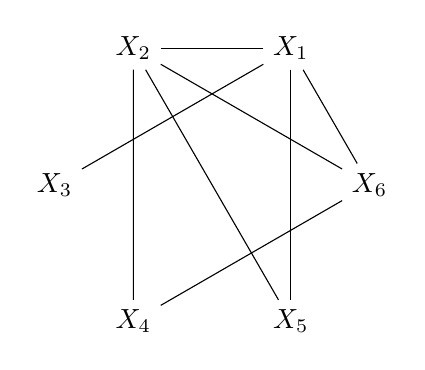
\begin{tikzpicture}
			      \foreach \x in {1, ..., 6} {
					      \node (X\x) at (60*\x:2) {$X_\x$};
				      }
			      \draw (X1) -- (X2);
			      \draw (X2) -- (X5);
			      \draw (X1) -- (X3);
			      \draw (X2) -- (X4) -- (X6) -- (X2) -- cycle;
			      \draw (X1) -- (X6);
			      \draw (X1) -- (X5);
		      \end{tikzpicture}
	      \end{center}

	      Conditioning on $X_1$ and $X_2$ using the theorems from class gives us the subgraph

	      \begin{center}
		      \begin{tikzpicture}
			      \foreach \x in {3, ..., 6} {
					      \node (X\x) at (60*\x:2) {$X_\x$};
				      }
			      \draw (X4) -- (X6);
		      \end{tikzpicture}
	      \end{center}

	      with disjoint components $\{X_3\}, \{X_5\}, \{X_4, X_6\}$. By a theorem from class, we know that this implies that $X_4$ and $X_6$ are conditionally independent from $X_3$ and $X_5$ given $X_1$ and $X_2$.
	      \color{black}
	      \pagebreak


	      %%%%%%%%%%%%%%%%%% Problems   %%%%%%%%%%%

	\item Suppose that $X=(X_1,\dotsc,X_6)$ respects the graph $G=(V,E)$ given by $V=\{X_1,\dotsc,X_6\}$ and
	      \[E=\{(X_1,X_2),(X_2,X_3),(X_3,X_4),(X_4,X_5),(X_5,X_6),(X_1,X_6),(X_3,X_6)\}.\]
	      \begin{enumerate}
		      \item Use the marginalization and conditioning rules to show
		            that the conditional distribution of $X_1,\dotsc,X_5$ given $X_6=x_6$ is a Markov chain, meaning that it respects the nearest-neighbor linear graph.

		            \color{blue}
		            We can draw the graph as follows:

		            \begin{center}
			            \begin{tikzpicture}
				            \foreach \x in {1, ..., 6} {
						            \node (X\x) at (60*\x:2) {$X_\x$};
					            }
				            \draw (X1) -- (X2) -- (X3) -- (X4) -- (X5) -- (X6) -- (X1);
				            \draw (X3) -- (X6);
			            \end{tikzpicture}
		            \end{center}

		            Conditioned on $X_6$, the distribution of $X_1,\dotsc,X_5$ is given by the subgraph $G \cap \{X_6\}^c$:

		            \begin{center}
			            \begin{tikzpicture}
				            \foreach \x in {1, ..., 5} {
						            \node (X\x) at (60*\x:2) {$X_\x$};
					            }
				            \draw (X1) -- (X2) -- (X3) -- (X4) -- (X5);
			            \end{tikzpicture}
		            \end{center}
		            which is just the nearest-neighbor linear graph.

		            \color{black}

		      \item
		            What is the simplest graph that $X_1,\ldots,X_5$ is guaranteed to respect?\footnote{A graph $G'$ would be ``guaranteed'' if it were respected by $X_1,X_2,\ldots,X_5$ for {\em every} distribution on
			            $X_1,X_2,\ldots,X_6$ which respects $G$. By ``simplest,'' there should be no graph with fewer edges that is also guaranteed to be respected.}

		            \color{blue}
		            \begin{center}
			            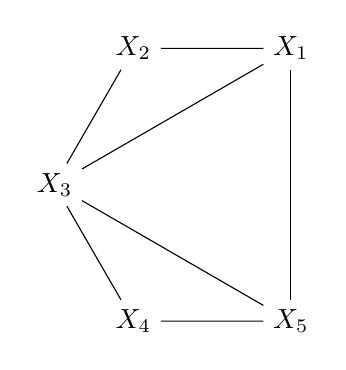
\begin{tikzpicture}
				            \foreach \x in {1, ..., 5} {
						            \node (X\x) at (60*\x:2) {$X_\x$};
					            }
				            \draw (X1) -- (X2) -- (X3) -- (X4) -- (X5);

				            \draw (X1) -- (X3) -- (X5);
				            \draw (X1) -- (X5);
			            \end{tikzpicture}
		            \end{center}
		            \color{black}



		      \item Is the conditional distribution of $X_1,\dotsc,X_4$ given $X_5=x_5$ necessarily a Markov chain?
		            In other words, does $X_{1:4}$, given $X_5$, necessarily respect the
		            nearest-neighbor linear graph?

		            \color{blue}
		            First, we need to marginalize $X_6$ out of the graph and then condition on $X_5$. The marginalized graph is precisely the simplest graph from part (b). Hence, we can draw the graph $(X_1, X_2, X_3, X_4 \; | \; X_5)$ as

		            \begin{center}
			            \begin{tikzpicture}
				            \foreach \x in {1, ..., 4} {
						            \node (X\x) at (60*\x:2) {$X_\x$};
					            }
				            \draw (X1) -- (X2) -- (X3) -- (X4);
				            \draw (X1) -- (X3);

			            \end{tikzpicture}

		            \end{center}

		            While the nearest neighbor linear graph is indeed a subgraph of the above, we do not have a guarantee that this is a Markov chain for every possible distribution on $(X_1, X_2, X_3, X_4)$.
		            \color{black}

	      \end{enumerate}

	      %%%%%%%%%%%%%%%%%% Problems  %%%%%%%%%%%


	      \pagebreak


	\item Consider the following joint pmf for the random variables $U,V,W,X,Y,Z$, each taking values in the finite set $\{1,\dotsc,L\}$:
	      \[ f(u,v,w,x,y,z) = \phi_1(u,v)\phi_2(u,v,w)\phi_3(w,x,y)\phi_4(x,z)\phi_5(x,y,z)\phi_6(u,z) \]
	      where $\phi_1,\dotsc,\phi_6$ are each nonnegative functions.
	      \begin{enumerate}
		      \item Do these variables respect the complete graph over 6 nodes?  Why or why not?

		            \color{blue}

		            Any distribution $p(x)$ for $x \in \R^n$ will be a GRF on the complete graph $K_n$. Hence, this distribution respects the complete graph.

		            \color{black}

		      \item Draw the simplest possible graph these variables are guaranteed to respect.

		            \color{blue}
		            We can draw the graph as follows:

		            \begin{center}
			            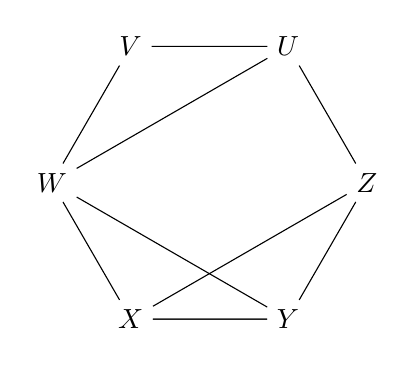
\begin{tikzpicture}
				            \foreach \x/\i in {U/1, V/2, W/3, X/4, Y/5, Z/6} {
						            \node (\x) at (60*\i:2) {$\x$};
					            }

				            \draw (U) -- (V) -- (W) -- (U) -- cycle;
				            \draw (W) -- (X) -- (Y) -- (W) -- cycle;
				            \draw (X) -- (Y) -- (Z) -- (X) -- cycle;
				            \draw (U) -- (Z);

			            \end{tikzpicture}
		            \end{center}

		            Trivially, if we were to remove any edge from the graph, we would not respect the maximum cliques of the pmf.
		            \color{black}

		      \item Are $U$ and $X$ necessarily independent?  Could they be independent?

		            \color{blue}
		            No. Lack of an edge does not imply independence. Consider the case $Z \sim \text{Bernoulli}(1/2)$ and
		            \[\begin{cases}
				            U, X \sim \text{Bernoulli}(0.01) & \text{if } Z = 1 \\
				            U, X \sim \text{Bernoulli}(0.99) & \text{if } Z = 0
			            \end{cases}\]

		            Then $U$ and $X$ do not share an edge, but they are also not independent.

		            However, we could also imagine a case where $U, X \overset{\text{iid}}{\sim} p$ and $Z = U + X$ in which case they would be independent.
		            \color{black}

		      \item Find a collection of variables (from the set $V,W,Y,Z$) such that $U$ and $X$ are necessarily conditionally independent given the values of these variables.  Your collection should have the fewest number of variables possible.  Justfy your choice or prove that no such collection necessarily exists.

		            \color{blue}
		            We can draw $(U, V, X, Y \; | \; W, Z) 	$ as
		            \begin{center}
			            \begin{tikzpicture}[node distance=2cm]
				            \node (V) at (0, 0) {$V$};
				            \node[right of=V] (U) {$U$};
				            \node[below of=V] (X) {$X$};
				            \node[below of=U] (Y) {$Y$};

				            \draw (U) -- (V);
				            \draw (X) -- (Y);

			            \end{tikzpicture}
		            \end{center}
		            in which case $U$ and $X$ are independent.

		            In any case where we were to remove only one vertex, we would still have a path between $U$ and $X$ in the subgraph. Hence, to guarantee independence, we need to remove at least two vertices.
		            \color{black}

	      \end{enumerate}

	      %%%%%%%%%%%%%%%%%%% Problems  %%%%%%%%%%%
	      %
	      %
	      %\item It sometimes happens that random variables can be transformed (without loss of information) into new random variables in such a way that the new random variables respect a much simpler graph.  Here is an elementary example of this.  
	      %
	      %Let $X=(X_1,\dotsc,X_m)$ have a joint distribution that is multinomial$(n;p_1,\dotsc,p_m)$, meaning that the joint pmf is
	      %\begin{equation} \label{e} \textstyle f(x_1,\dotsc,x_m) \triangleq n!\ind\bigl\{\sum_{j=1}^m x_j=n\bigr\}\displaystyle\prod_{i=1}^m\frac{p_i^{x_i}}{x_i!}\ind\bigl\{x_i\in\{0,1,\dotsc,n\}\bigr\} \end{equation}
	      %for a nonnegative integer $n$ and for nonegative $p_1,\dotsc,p_m$ with $\sum_{i=1}^m p_i =1$.  Here's how the multinomial arises.  Consider $n$ iid trials $Y_1,\dotsc,Y_n$, where each $Y_k\in\{1,2,\dotsc,m\}$ with respective probabilities $p_1,\dotsc,p_m$ that sum to one.  In other words, on each trial exactly one of $m$ distinct things can happen.  Let $X_i$ be the number of times that $i$ happens in the $n$ trials, that is,
	      %\[  \textstyle X_i \triangleq \sum_{k=1}^n\ind\{Y_k=i\} \]
	      %Then the joint distribution of $(X_1,\dotsc,X_m)$ is multinomial$(n;p_1,\dotsc,p_m)$.
	      %\be
	      %\item Assume that $p_i>0$, for $i=1,\ldots,m$.
	      %A quick glance at the representation in \eqref{e} does not reveal how to further factor $\ind\bigl\{\sum_{j=1}^m x_j=n\bigr\}$, so it seems that $X$ only respects the complete graph.  Of course, maybe there is some way to factor this term that we are not thinking about, in which case $X$ might respect a simpler graph.  Prove that the complete graph is the only graph that $X$ respects.  Hint: Think about how the multinomial arises and argue that no $X_i$ and $X_j$ can be conditionally independent given the rest of the $X_k$'s.
	      %\item Define the new random variables $S=(S_1,\dotsc,S_m)$ by
	      %\[ \textstyle S_k \triangleq \sum_{i=1}^k X_i \]
	      %These are the partial sums of the $X_i$'s.  Show that the transformation from $X$ to $S$ is invertible (meaning that you can recover $X$ from just $S$).  Show that $S$ is a Markov chain: $S$ respects a graph which only has edges $\{k,k+1\}$, $k=1,\ldots,m-1$.
	      %\ee

	      %%%%%%%%%%%%%%%%%% Problems  %%%%%%%%%%%

	      \pagebreak

	\item {\bf Proof of the conditioning rule for Gibbs random fields.} Let $X=(X_1,\dotsc,X_d)$ be a random vector over a discrete space.  Suppose that $X$ respects the graph $G$.
	      Assume that $\Prob(X_{A^c}=x_{A^c})>0$.
	      Prove that the conditional distribution on $X_A$ given $X_{A^c}=x_{A^c}$ (i.e. $X_A|X_{A^c}=x_{A^c}$) respects the subgraph of $G$ over the vertices in $A$.

	      \color{blue}
	      By a slight abuse of notation,
	      \begin{align*}
		      f(x_A \; | \; x_{A^c}) & = \frac{f(x_A,x_{A^c})}{f(x_{A^c})}                                                                                                \\
		                             & = \frac{f(x)}{f(x_{A^c})}                                                                                                          \\
		                             & = \frac{\frac{1}{Z} \prod_{i \sub A} \phi_i(x_i) \prod_{\begin{subarray}{c}
					                                                                                       j \sub G\\
					                                                                                       j \not\sub A^c, j \not\sub A
				                                                                                       \end{subarray}} \phi_j(x_j)}{\frac{1}{Z'} \prod_{k \sub A^c} \phi_k(x_k) } \\
	      \end{align*}

	      However, since $A^c$ is fixed, each $\phi_j(x_j)$ will be only a function of $x \in A$, hence included already in the first product. Therefore, we can write
	      \[f(x_A \; | \; x_{A^c}) = \frac{\frac{1}{Z} \prod_{i \sub A} \phi_i(x_i) \prod_{j \sub A^c} \phi_j(x_j)}{\frac{1}{Z'} \prod_{k \sub A^c} \phi_k(x_k) } = \frac{1}{Z''} \prod_{i \sub A} \phi_i(x_i)\]
	      which respects the graph $G \vert_A$.
	      \color{black}


	      \pagebreak



	\item[] \hspace{-3ex} {\bf For 2610 or for extra credit:}





	      %%%%%%%%%%%%%%%%%%%%%%%%%%
	      %			Problem  
	      %%%%%%%%%%%%%%%%%%%%%%%%%%

	      %	
	      %	\item {\bf The RBF is positive definite.} Prove that the Gaussian radial basis function kernel is positive definite in the following cases. (You will get a lot of partial credit for proving nonnegative definite.)
	      %	\be 
	      %	\item Prove it for dimension $d=1$. Hint: Write $\kappa(u,v)=g(u-v)$.  Expand $g$ as a Fourier transform, so that $g$ becomes an integral.  Now use this representation to show positive definiteness.  You may look up the formula for the characteristic function of a Gaussian random variable in order to simplify a lot of the calculus.    
	      %	\item Prove it for any finite $d$.
	      %	\ee




	      %%%%%%%%%%%%%%%%%%%%%%%%%%
	      %			Problem 
	      %%%%%%%%%%%%%%%%%%%%%%%%%%


	\item {\bf Two formulations of the maximum-margin problem.}

	      Let $x_1,\ldots,x_n\in \mathds{R}^d$  and let $y_1,\ldots,y_n \in \{-1,1\}$.
	      Assume that $\{(x_i,y_i)\}_{i=1:n}$ is consistent (i.e. $x_i=x_j \Rightarrow y_i=y_j$) and linearly separable.
	      (Any pair, $\alpha\in\mathds{R}^1$ and $\beta\in\mathds{R}^d$, defines a classifier, $h(x)$: $h(x)\triangleq \text{sign}\left(\alpha + \beta\cdot x \right)$.)


	      The goal is to show that the following two formulations of the problem of finding a maximum margin classifier were equivalent:

	      \begin{enumerate}[(i)]
		      \item
		            Find $\hat{\alpha}$, $\hat{\beta}$, and $\hat{M}$ to solve
		            \[
			            \text{argmax}_{M,\alpha,\beta:\|\beta\| = 1} M \qquad
			            \text{subject to}\ \ y_k\left(\alpha + \beta\cdot x_k\right) \geq M\quad \forall\ k=1:n
		            \]
		      \item
		            Find $\hat{\alpha}$ and $\hat{\beta}$ to solve
		            \[
			            \argmin_{\alpha,\beta} \frac{1}{2}\sum_{i=1}^d \beta^2 \qquad
			            \text{subject to}\ \ y_k\left(\alpha + \beta\cdot x_k\right) \geq 1\quad \forall\ k=1:n
		            \]


	      \end{enumerate}

	      Construct a transformation from a solution to (i) into a solution to (ii), and another transformation from a solution to (ii) into a solution to (i).


	      \pagebreak

	      %%%%%%%%%%%%%%%%%%%%%%%%%%
	      %			Problem  
	      %%%%%%%%%%%%%%%%%%%%%%%%%%

	      %	
	      %	\item {\bf Persistence of perfect classification?}
	      %	\label{item:Persistence}
	      %	This is a continuation of problem (\ref{item:two_losses}). 
	      %	Suppose that we are training by continuous gradient descent, and at some point during training the error rate is zero. 
	      %	
	      %	Show or produce a counter example:  if we continue to train by continuous gradient descent, then the error rate will continue to be zero.
	      %	
	      %
	\item {\bf Proof of the marginalizing rule for Gibbs random fields.} Let $X=(X_1,\dotsc,X_d)$ be a random vector over a discrete space.  Suppose that $X$ respects the graph $G$.  Prove that $X_A$ respects the graph $G'$ over the vertices in $A$, where $i$ and $j$ are connected in $G'$ if they are directly connected in $G$ or if there is a path from $i$ and $j$ completely within $A^c$ in $G$.

	      %%%%%%%%%%%%%%%%%%%%%   %%%%%%%%%%%%%%%%%%%%%%%

	      \pagebreak


	\item {\bf Equivalence of two-sided and one-sided Markov properties for positive pmfs.} Let $X=(X_1,\dotsc,X_d)$ be a random vector over a discrete space. The familiar ``one-sided Markov property'' is
	      \[ \Prob(X_t=x_t|X_{1:t-1}=x_{1:t-1}) = \Prob(X_t=x_t|X_{t-1}=x_{t-1}) \]
	      for all $x$ and each $t=1,\dotsc,d$.\footnote{Interpreted as  $\Prob(X_1=x_1)=\Prob(X_1=x_1)$, when $t=1$.} The ``two-sided Markov property'' is
	      \[ \Prob(X_t=x_t|X_{1:t-1}=x_{1:t-1},X_{t+1:d}=x_{t+1:d}) = \Prob(X_t=x_t|X_{t-1}=x_{t-1},X_{t+1}=x_{t+1}) \]
	      for all $x$ and each $t=1,\dotsc,d$.\footnote{Interpreted as $\Prob(X_1=x_1|X_{2:d}=x_{2:d}) = \Prob(X_1=x_1|X_2=x_2)$ when $t=1$, and $\Prob(X_d=x_d|X_{1:d-1}=x_{1:d-1}) = \Prob(X_d=x_d|X_{d-1}=x_{d-1})$ when $t=d$.} Prove that these two properties are equivalent as long as $X$ has a strictly positive pmf. You can assume the independence, conditioning, and marginalizing rules for GRFs, and can use the Hammersley-Clifford theorem. (It is also instructive to try to prove it without the Hammersley-Clifford theorem. It is surprisingly hard.)



\end{enumerate}

\end{document}